 %%%%%%%%Added
\documentclass [xcolor=svgnames] {beamer} 
\usepackage[utf8]{inputenc}
\usepackage{booktabs, comment} 
\usepackage[absolute, overlay]{textpos} 
\useoutertheme{infolines} 
\setbeamercolor{title in head/foot}{bg=internationalorange}
\setbeamercolor{author in head/foot}{bg=dodgerblue}
\usepackage{xcolor}
\usetheme{Boadilla}
\setbeamercovered{invisible}
\setbeamertemplate{navigation symbols}{}
\definecolor{myuniversity}{RGB}{0, 60, 113}
\definecolor{internationalorange}{RGB}{231, 93,  42}
\definecolor{dodgerblue}{RGB}{0, 119,202}
\usecolortheme[named=myuniversity]{structure}


\usepackage{colortbl}
\usepackage{color}
\usepackage{color, colortbl}
\usepackage[table]{xcolor}
\usepackage{wrapfig}
\usepackage{algorithmic}
\usepackage{algorithm}
\usepackage{latexsym}
\usepackage{graphicx}
\usepackage{times}
\usepackage{amssymb}
\usepackage{geometry}                                        
\usepackage{tikz}
\usepackage{pgf}
\usepackage{hyperref}
\usepackage{subfig}

\logo{\pgfputat{\pgfxy(0,8)}{\pgfbox[right,base]{\includegraphics[height=0.73cm]{logo.png}}}}


\usepackage[square, sort, numbers, authoryear]{natbib}
\bibliographystyle{plain}
%\addbibresource{ref.bib}

\title[AFQ-IoT]{\textbf{AFQ-IoT: Adaptive, Federated, and Quantum-Resistant AI-Blockchain IoT Framework}}

\author[Shiva, Akshay, Ashish (IIIT-H)]{
    \textbf{Presented By}\\
    \textbf{Shiva Shankar} (2023202005) \\ \texttt{shivashankar.gande@students.iiit.ac.in} \\[0.2\baselineskip]
    \textbf{Akshay Kohad} (2023202007) \\ \texttt{akshay.kohad@students.iiit.ac.in} \\[0.2\baselineskip]
    \textbf{Ashish Lakhmani} (2023202008) \\ \texttt{ashish.lakhmani@students.iiit.ac.in}
}

\institute[]
{
    \vspace{0.5cm} % Adjusted space for fitting
    \large \textbf{International Institute of Information Technology, Hyderabad}
}

\date{November 5, 2024}



\begin{document}

%------------------------------------------------
%	TITLE FRAME
%------------------------------------------------
\begin{frame}
\titlepage
\end{frame}

%------------------------------------------------
%	OUTLINE FRAME
%------------------------------------------------
\begin{frame}
\frametitle{Outline}
  \tableofcontents
\end{frame}


\section{Introduction}
%------------------------------------------------
%	SECTION 1a: INTRODUCTION (Background)
%------------------------------------------------
\begin{frame}
\small
\frametitle{Introduction: Background}
\subsection{Background}

\begin{itemize}
\item This paper discusses how the Internet of Things (IoT) connects various devices, such as smart homes and vehicles, to the internet, creating an interconnected network known as the Internet of Everything (IoE). 

\item While IoT is beneficial in improving productivity across multiple fields, it faces challenges like big data analytics, security, and centralization issues. 

\item To tackle these challenges, this paper suggests integrating both Artificial intelligence (AI) and Blockchain technology. IoT generates a huge mass of data, but AI assists in processing this data, and Blockchain offers secure and decentralized data storage. The aim of this collaboration is to establish a more secure, efficient, and scalable IoT framework, which is essential in addressing the existing challenges in data management and security.
\end{itemize}

\end{frame}


%------------------------------------------------
%	SECTION 1b: INTRODUCTION (Network Model)
%------------------------------------------------
\begin{frame}[allowframebreaks]
\small
\frametitle{Introduction: Network Model}
\subsection{Network Model}

\begin{center}
    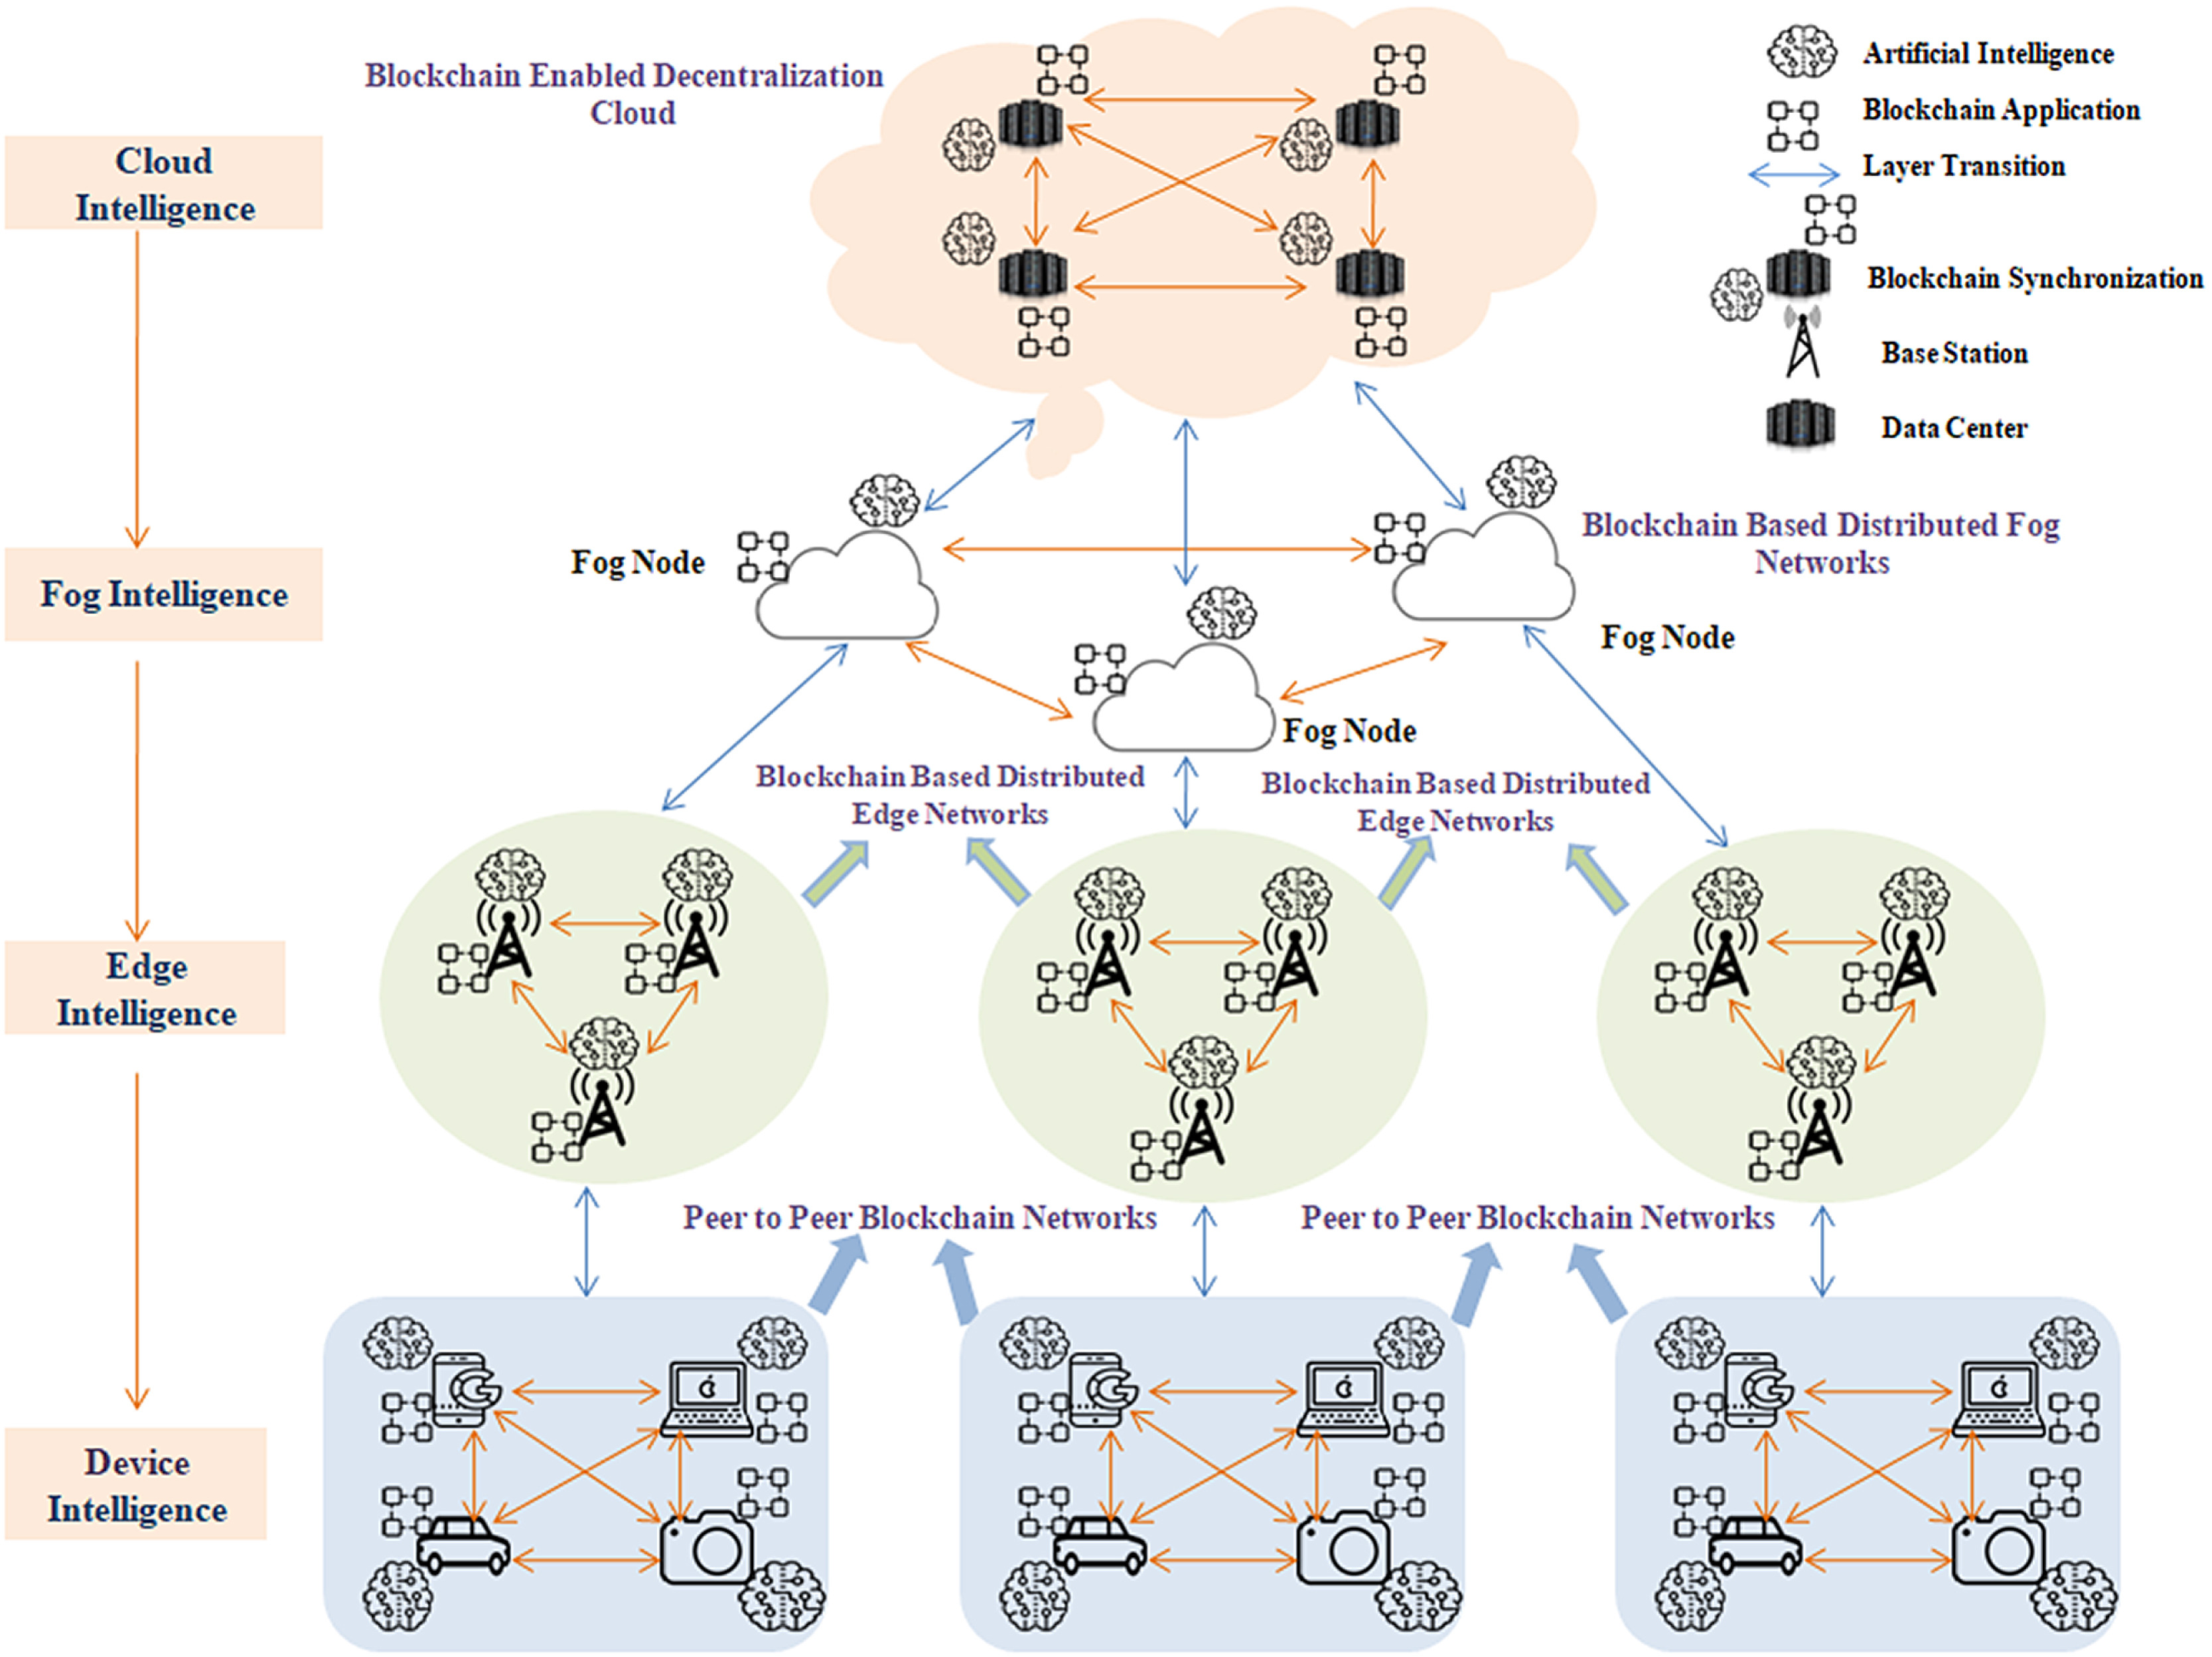
\includegraphics[width=0.80\textwidth]{blockIOTIntelligence.jpg} % Replace with your image path
\end{center}

\begin{itemize}
\item \textbf{Device Intelligence:} \textbf{Role}: Data collection from IoT devices and sensors, \textbf{AI}: Local pre-processing and basic pattern recognition, \textbf{Blockchain}: Peer-to-peer security and privacy for direct device interactions.

\item \textbf{Edge Intelligence:} \textbf{Role}: Initial data aggregation and processing from devices, \textbf{AI}: Feature extraction and data filtering close to the source, \textbf{Blockchain}: Secure, decentralized communication for efficient data handling at the edge.

\item \textbf{Fog Intelligence:} \textbf{Role:} Intermediate layer for larger-scale data processing and decision-making, \textbf{AI:} Advanced data analysis and machine learning model training, \textbf{Blockchain:} Distributed ledger for secure, decentralized data management, addressing scalability.
    
\item \textbf{Cloud Intelligence:} \textbf{Role:} Centralized, high-level data storage and analysis, \textbf{AI:} Intensive big data analysis in cloud data centers, \textbf{Blockchain:} Decentralized data storage for secure, scalable access and archival of IoT data.
\end{itemize}

\end{frame}



%------------------------------------------------
%	SECTION 1c: INTRODUCTION (Attack Model)
%------------------------------------------------
\begin{frame}
\normalsize
\frametitle{Introduction: Attack Model}
\subsection{Attack Model}

\begin{itemize}
\item \textbf{Data Breaches}: Blockchain’s cryptographic methods ensure data confidentiality, limiting access to authorized parties.

\item \textbf{Malware and Unauthorized Access}: Blockchain’s immutable ledger logs all transactions, preventing data tampering and unauthorized modifications.

\item \textbf{Data Tampering}: The decentralized consensus mechanism of Blockchain ensures any data changes are transparent and verifiable.

\item \textbf{Centralization Vulnerabilities}: By decentralizing data storage, Blockchain reduces reliance on a single server, enhancing resilience against DDoS and single-point failures.
\end{itemize}

\end{frame}


%------------------------------------------------
%	SECTION 1d: INTRODUCTION (Research Contribution)
%------------------------------------------------
\begin{frame}
\normalsize
\frametitle{Introduction: Research Contribution}
\subsection{Research Contribution}
\begin{itemize}

\item Privacy-Preserving Federated Learning for IoT Devices
\item Quantum-Resistant Cryptographic Security
\item Adaptive Consensus Mechanism for Efficient Resource Utilization
\item Cross-Chain Compatibility for Multi-Domain Interoperability
\item Localized Blockchain and Distributed AI for Enhanced Edge Processing
\item Federated Trust Mechanism for Secure Collaborative Anomaly Detection
\item Energy-Efficient Quantized AI Models for Scalable Large-Scale Analysis

\end{itemize}
\end{frame}


\section{Literature Review}
%------------------------------------------------
%	SECTION 2: LITERATURE REVIEW
%------------------------------------------------
\begin{frame}[allowframebreaks]
\small
\frametitle{Literature Review}

\begin{itemize}
\item \textbf{Rathore et al. (2019):}\\
\textbf{Focus: }Blockchain and deep learning (DL) integration for secure IoT.\\
\textbf{Contribution: }Blockchain-secured DL model for data privacy and decentralized security.\\
\textbf{Limitation: }Limited scope on Blockchain-AI integration for broader IoT applications.

\item \textbf{Atlam et al. (2018):}\\
\textbf{Focus: }AI-IoT integration for data security and analysis\\
\textbf{Contribution: }Framework improving data privacy with AI in IoT.\\
\textbf{Limitation: }Lacks emphasis on Blockchain’s role.

\item \textbf{Wright et al. (2018):}\\
\textbf{Focus: }Integration of Blockchain and AI to address scalability and data processing in IoT.\\
\textbf{Contribution: }Proposed a hybrid architecture using Blockchain’s decentralized ledger and AI to optimize data flow and efficiency in IoT.\\
\textbf{Limitation: }Limited focus on security and privacy; lacked application across multi-layered IoT architectures like fog and cloud.

\item \textbf{Qian et al. (2018):}\\
\textbf{Focus: }IoT network security.\\
\textbf{Contribution: }Blockchain-based network security for traffic monitoring and identity verification.\\
\textbf{Limitation: }Minimal focus on AI.

\item \textbf{Xu et al. (2017):}\\
\textbf{Focus: }Decentralized IoT resource management.\\
\textbf{Contribution: }Blockchain framework for efficient resource handling and scalability.\\
\textbf{Limitation: }Limited exploration of AI for IoT data analysis.

\item \textbf{Zheng et al. (2017):}\\
\textbf{Focus: }Taxonomy of Blockchain technologies.\\
\textbf{Contribution: }Classification of Blockchain types and consensus algorithms relevant to IoT.\\
\textbf{Limitation: }No emphasis on AI-Blockchain integration for IoT.
\end{itemize}

\end{frame}


\section{Summary of Techniques}
%------------------------------------------------
%	SECTION 3: SUMMARY OF TECHNIQUES
%------------------------------------------------
\begin{frame}
\scriptsize
\frametitle{Summary of Techniques}

\setlength{\tabcolsep}{5pt} % Adjust horizontal padding
\renewcommand{\arraystretch}{2} % Adjust vertical padding

\begin{table}[h!]
\centering
\begin{tabular}{|>{\raggedright\arraybackslash}m{2cm}|>{\raggedright\arraybackslash}m{3cm}|>{\raggedright\arraybackslash}m{3cm}|>{\raggedright\arraybackslash}m{2cm}|}
\hline
\textbf{Research Work} & \textbf{Techniques Used} & \textbf{Advantages} & \textbf{Disadvantages} \\
\hline
Rathore et al. (2019) & Blockchain + DL & Privacy, Decentralized Security & Limited IoT Integration \\
\hline
Atlam et al. (2018) & AI + IoT & Data Privacy, Analysis & Minimal Blockchain Focus \\
\hline
Xu et al. (2017) & Blockchain for Resource Management & Scalability, Efficiency & Limited AI Use \\
\hline
Qian et al. (2018) & Blockchain for Network Security & Identity Verification, Security & Minimal AI Application \\
\hline
Zheng et al. (2017) & Blockchain Taxonomy & Detailed Blockchain Overview & Lacks AI-IoT Focus \\
\hline
Wright et al. (2018) & Hybrid Blockchain + AI & Scalability, Data Flow & Limited Security, No Multi-layer IoT \\
\hline
\end{tabular}
\label{table:litreview}
\end{table}

\end{frame}



\section{Proposal}
%------------------------------------------------
%	SECTION 4a: PROPOSAL (Motivation)
%------------------------------------------------
\begin{frame}
\small
\subsection{Motivation}
\frametitle{Proposal: Motivation}
In the following paper titled "BlockIoTIntelligence: A Blockchain-enabled Intelligent Internet of Things Architecture Based on Artificial Intelligence" we will see a framework that integrates blockchain with AI to solve the critical IoT problems of centralization, security, and latency. That said, there are still challenges, especially regarding AI energy efficiency, interoperability, data management, and privacy. This shows us that we have to enhance the BlockIoTIntelligence model to indeed be flexible, sustainable and privacy delinquent to be feasible for broader use cases in the real IoT world. To tackle these issues, we propose an updated architecture, called AFQ-IoT with : 
\begin{itemize}
\item Federated Learning for Privacy and Efficiency
\item Adaptive AI-Driven Consensus Mechanism
\item Cross-Chain Compatibility for Interoperability
\item Quantum-Resistant Cryptography for Future-Proof Security
\item  Adaptive AI Models for Real-Time Decision Making
\end{itemize}

\end{frame}


%------------------------------------------------
%	SECTION 4b: PROPOSAL (Proposed Solution)
%------------------------------------------------
\begin{frame}[allowframebreaks]
\footnotesize
\subsection{Proposed Solution}
\frametitle{Proposal: Proposed Solution}

\begin{itemize}

\item \textbf{Federated Learning for Privacy and Efficiency}:\\
\textbf{Objective}: Protect data privacy and reduce IoT network energy use.\\
\textbf{Approach}: Train AI models locally on devices, sharing only model updates instead of raw data.\\
\textbf{Justification}: Reduces data transfer and keeps sensitive info on devices, ideal for privacy-sensitive fields like healthcare.

\item \textbf{Adaptive AI-Driven Consensus Mechanism}:\\
\textbf{Objective}: To cut down on Blockchain for IoT energy consumption.\\
\textbf{Approach}: Eliminate Proof of Work (PoW) and find less energy intensive methods like PoS and DPoS.\\
\textbf{Justification}: Scales Blockchain for IoT’s energy constrained environment, notably in case of massive networks.

\item \textbf{Cross-Platform Interoperability}:\\
\textbf{Objective}: Ensure Cross Ecosystem Integration of IoT Devices.\\
\textbf{Approach}: Include basic compatible protocol and middleware (Zigbee, MQTT, LoRaWAN. etc.).\\
\textbf{Justification}: It breaks down barriers between systems, allowing BlockIoTIntelligence to become more flexible and support more IoT devices.

\item \textbf{Quantum-Resistant Cryptography for Long-Term Security}:\\
\textbf{Objective}: Safeguard IoT data and transactions from future quantum-based threats.\\
\textbf{Approach}: Use quantum-resistant algorithms, like lattice-based cryptography, within the blockchain.\\
\textbf{Justification}: Traditional encryption could be broken by quantum computing. Quantum-resistant cryptography ensures lasting data security, essential for areas like finance and healthcare that need ongoing data protection.

\item \textbf{Adaptive AI Models for Real-Time Decision Making }:\\
\textbf{Objective}: To extend responsiveness and international decision making precision.\\
\textbf{Approach}: Employ adaptive models such as reinforcement learning or transfer learning to rapidly adapt to incoming variations in data and network scenarios.\\
\textbf{Justification}: Provides the ability to respond in real time, which is important in applications where you want to receive immediate insights (e.g., traffic or predictive maintenance).
\end{itemize}

\end{frame}


\section{Analysis}
%------------------------------------------------
%	SECTION 5a: ANALYSIS (Security Analysis)
%------------------------------------------------
\begin{frame}
\footnotesize
\subsection{Security Analysis}
\frametitle{Analysis: Security Analysis}

\begin{itemize}
\item \textbf{Federated Learning for Privacy: }\\
It enables local AI model training on IoT devices and shares only model updates which protect sensitive data and reduce privacy risks.

\item \textbf{Adaptive AI-Driven Consensus: }\\
Adjusts blockchain protocols based on network risk levels—switching to secure protocols like Proof-of-Stake (PoS) in high-risk situations and conserving resources with Proof-of-Authority (PoA) during low-risk times.

\item \textbf{Cross-Chain Compatibility: }\\
Facilitates secure data exchange across IoT domains, preventing data silos and enabling verified, authorized data sharing for sensitive, multi-domain applications.

\item \textbf{Quantum-Resistant Blockchain: }\\
Uses quantum-safe cryptography to secure IoT data against future quantum-based threats, ensuring long-term transaction security.

\item \textbf{Quantum-Resistant Smart Contracts: }\\
Enforces access control with quantum-safe smart contracts, securing data integrity and regulatory compliance by ensuring only authorized access to critical IoT data.
\end{itemize}

\end{frame}


%------------------------------------------------
%	SECTION 5b: ANALYSIS (Communication Analysis)
%------------------------------------------------
\begin{frame}
\footnotesize
\subsection{Communication Analysis}
\frametitle{Analysis: Communication Analysis}

\begin{itemize}
\item \textbf{Federated Learning and Reduced Data Transmission: }\\
Federated Learning and Less Data Transmission Federated learning at the device level is leveraged to reduce the amount of data sent up to central nodes in the AFQ-IoT. It reduces the communication complexity by sending only model updates(sliced data) to upper layers rather than slice data. This design saves bandwidth and improves privacy.

\item \textbf{Cross-Chain Protocols for Inter-Domain Communication: }\\
With fog layer cross-chain compatibility enables secure sharing data across different IoT domains without creating any bottleneck. This decentralised method lessens the communication needs between layers through localised exchanges of data and thereby reduces the overall communication burden of the system.

\item \textbf{Localized Blockchain for Efficient Data Verification: }\\
he edge layer employs a localized blockchain, allowing data verification to happen mostly within the edge layer and minimizing data transfer to the cloud layer. The processing done here minimizes latency and instead of system to system which make it suitable for time require IoT applications and improves the response times.

\end{itemize}

\end{frame}

%------------------------------------------------
%	SECTION 5c: ANALYSIS (Computation Analysis)
%------------------------------------------------
\begin{frame}
\footnotesize
\subsection{Computation Analysis}
\frametitle{Analysis: Computation Analysis}

\begin{itemize}
\item \textbf{Quantized AI Models: }\\
The cloud layer uses smaller, optimized AI models to process large IoT data quickly and with less computing power, essential for real-time, large-scale analysis.

\item \textbf{Adaptive Consensus Mechanism: }\\
It can alter the protocols of a blockchain based on its load. During low load periods, simpler protocols (PoA, etc.) are used and more complex protocols (PoS, etc.) during high load periods. This adaptive mechanism enables the crypto network to save energy and computational resources.

\item \textbf{Distributed AI in Fog Layer: }\\
It is responsible for local resource allocations on the devices which results in less bottleneck as devices will be able to share their workloads effectively, hence contributing to their overall functionality and for making them lesser dependent on centralized servers.

\item \textbf{Quantum-Resistant Cryptography:}\\
It selectively employs secure cryptography only at the device layer at the level of critical transactions while introducing minimal compute overhead and no degradation of performance.


\end{itemize}

\end{frame}


\section{Future Research Directions}
%------------------------------------------------
%	SECTION 6: Future Research Directions
%------------------------------------------------
\begin{frame}
\large
\frametitle{Future Research Directions}

\begin{itemize}
\item Development of Lightweight Quantum-Resistant Cryptographic Protocols
\item Adaptive Federated Learning with Real-Time Model Update Mechanisms
\item Integration of Edge AI for Enhanced Local Processing and Reduced Latency
\item Exploration of Secure AI Model Aggregation Techniques
\item Investigation of Self-Healing Mechanisms for IoT Networks
\end{itemize}

\end{frame}

%------------------------------------------------
%	References
%------------------------------------------------
\begin{frame}[allowframebreaks]
\scriptsize
\frametitle{References}
\begin{itemize}
    \item[1] S. Rathore, Y. Pan, J.H. Park, "BlockDeepNet: A blockchain-based secure deep learning for IoT network," \textit{Sustainability}, vol. 11, 2019, p. 3974. \url{http://dx.doi.org/10.3390/11143974}.
    \item[2] H.F. Atlam, R.J. Walters, G.B. Wills, "Intelligence of things: opportunities and challenges," in \textit{3rd Cloudification of the Internet of Things (CIoT)}, 2018, pp. 1–6. \url{http://dx.doi.org/10.1109/CIOT.2018.8627114}.
    \item[3] K.L. Wright, M. Espinoza, U. Chadha, B. Krishnamachari, "SmartEdge: A smart contract for edge computing," in \textit{IEEE International Conference on Internet of Things (iThings), Green Computing and Communications (GreenCom), Cyber, Physical and Social Computing (CPSCom), Smart Data (SmartData)}, 2018. \url{https://ieeexplore.ieee.org/document/8726601}.
    \item[4] Z. Zheng, S. Xie, H.N. Dai, X. Chen, H. Wang, "Blockchain challenges and opportunities: a survey," \textit{International Journal of Web Grid Services}, vol. 14, no. 4, 2018, pp. 352–375.
    \item[5] Y. Qian, Y. Jiang, J. Chen, Y. Zhang, J. Song, M. Zhou, M. Pustišek, "Towards decentralized IoT security enhancement: A blockchain approach," \textit{Computers and Electrical Engineering}, vol. 72, 2018, pp. 266–273. \url{https://www.sciencedirect.com/science/article/pii/S0045790618300508}.
    \item[6] C. Xu, K. Wang, M. Guo, "Intelligent resource management in blockchain-based cloud datacenters," \textit{IEEE Cloud Computing}, vol. 4, no. 6, 2017, pp. 50–59. \url{http://dx.doi.org/10.1109/MCC.2018.1081060}.
\end{itemize}
\end{frame}


%------------------------------------------------
%	Thankyou
%------------------------------------------------
\begin{frame}
  \begin{center}
    \textbf{\Huge Thank you very much!}\\
  \end{center}
\end{frame}
    
% End of slides
\end{document} 

